\section{Analyse de l'existant}
\subsection{le logiciel R}
\paragraph{}

Le logiciel R est à la fois un environnement interactif de calcul, en lignes de
commandes, et un langage de programmation. Il existe sur différentes plateformes
(Linux, MacOS et Windows). Il peut être utilisé pour des traitements de données
ou des analyses statistiques. R est un logiciel libre, ouvert à la participation de
développeurs extérieurs. En effet, l’environnement s’enrichit par l’intégration de
packages provenant de la communauté ajoutant des modules et des fonctionnalités
complémentaires au logiciel initial.\\\\

\begin{center}

\includegraphics[scale=0.7]{Rlogo.png}\\
\textit{Le logiciel R}
\end{center}

\paragraph{}
La communauté R est très active et de nombreux modules sont régulièrement proposés.
R permet facilement de charger des données, de sortir des informations statistiques, de visualiser
diverses courbes extraites des données, etc.
\paragraph{}
Par défaut, R se présente sous la forme d'une ligne de commande. Il est cependant possible de
développer des interfaces utilisateur pour contrôler l'application ainsi que pour visualiser des
résultats de traitement.

\begin{center}
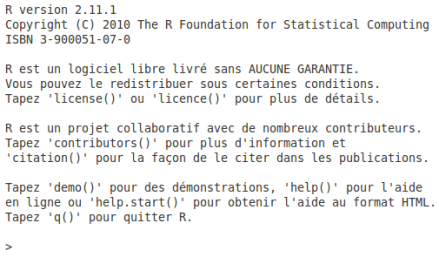
\includegraphics[scale=0.7]{demarrage_r.png}\\
\textit{Aperçu de la console R}
\end{center}
\newpage
\paragraph{} 
Le logiciel R nous permet de traiter des données tabulaires, sous forme de vecteurs, ou de data-frame (matrice contenant les instances de objets en ligne, avec un attribut par colonne). Il propose ensuite des opérations sur les vecteurs, tout en discriminant les objets par leurs attributs non numériques. Ce qui permet d’étiqueter les objets avant de faire des calculs et pouvoir ensuite différencier les résultats des calculs en fonction des étiquettes des objets.

\paragraph{} On utilisera sans doute cette particularité pour colorer les objets dans la fenêtre 3D, en fonction de leurs propriétés.

\newpage

\subsection{Le logiciel Explorer3D}
\paragraph{}
De leur coté, Matthieu Exbrayat et Lionel Martin, maîtres de conférences au Laboratoire d'informatique Fondamentale d'Orléans, développent depuis plusieurs années un logiciel de visualisation de données
doté d'une interface graphique 3D interactive. Ce logiciel est écrit en Java.\\
http://www.univ-orleans.fr/lifo/software/Explorer3D/

\begin{center}
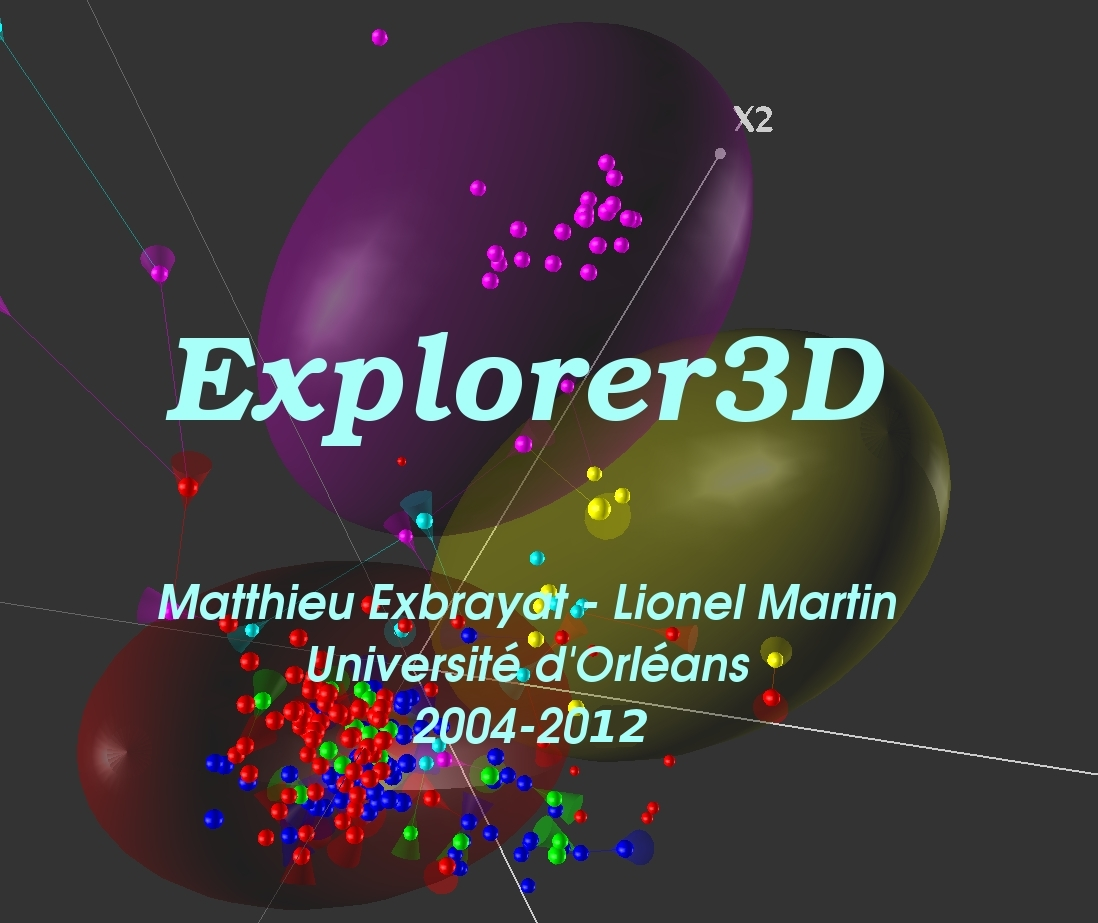
\includegraphics[scale=0.3]{explorer3d.jpg}\\
\textit{Explorer3D}
\end{center}

\paragraph{}
Ils ont acquis une bonne maîtrise de la structuration d'un tel outil afin de le rendre évolutif. Ils ont également mis en place un certain nombre de fonctionnalités interactives.
\newpage

\paragraph{} La plateforme R est devenue un standard du domaine de la classification. Mais le logiciel Explorer3D, propose une interface inédite pour la visualisation des résultats de classification. C'est pourquoi ses concepteurs souhaiteraient porter leur travail sous R, car ils sera ainsi plus facile d'accès et s'inscrira dans le standard du domaine. Cette mise aux normes du standard devrait permettre une diffusion plus large du projet Explorer3D, puisque cela le rendra utilisable par tous les utilisateurs de R.

\paragraph{}
Nous étudions maintenant les possibilités d'interactions entre ce logiciel et la plateforme R, afin d'intégrer rapidement divers outils existant sous R, mais également de diffuser notre logiciel vers cette communauté.\\
Au moins deux approches sont possibles :
\begin{itemize}
\item intégrer des invocations de R depuis java.
\item migrer notre logiciel vers R.
\end{itemize}

\paragraph{}
Concernant le premier point, l'invocation de R depuis java est relativement simple. Elle ne sera pas
abordée dans ce TER. Concernant le second point, R propose la création de fenêtres de contrôle et
de fenêtres graphiques 2D et 3D (voir par exemple http://rgl.neoscientists.org/). Toutefois, nous ne
connaissons pas les possibilités d'interaction réelles de l'interface 3D.

\begin{center}
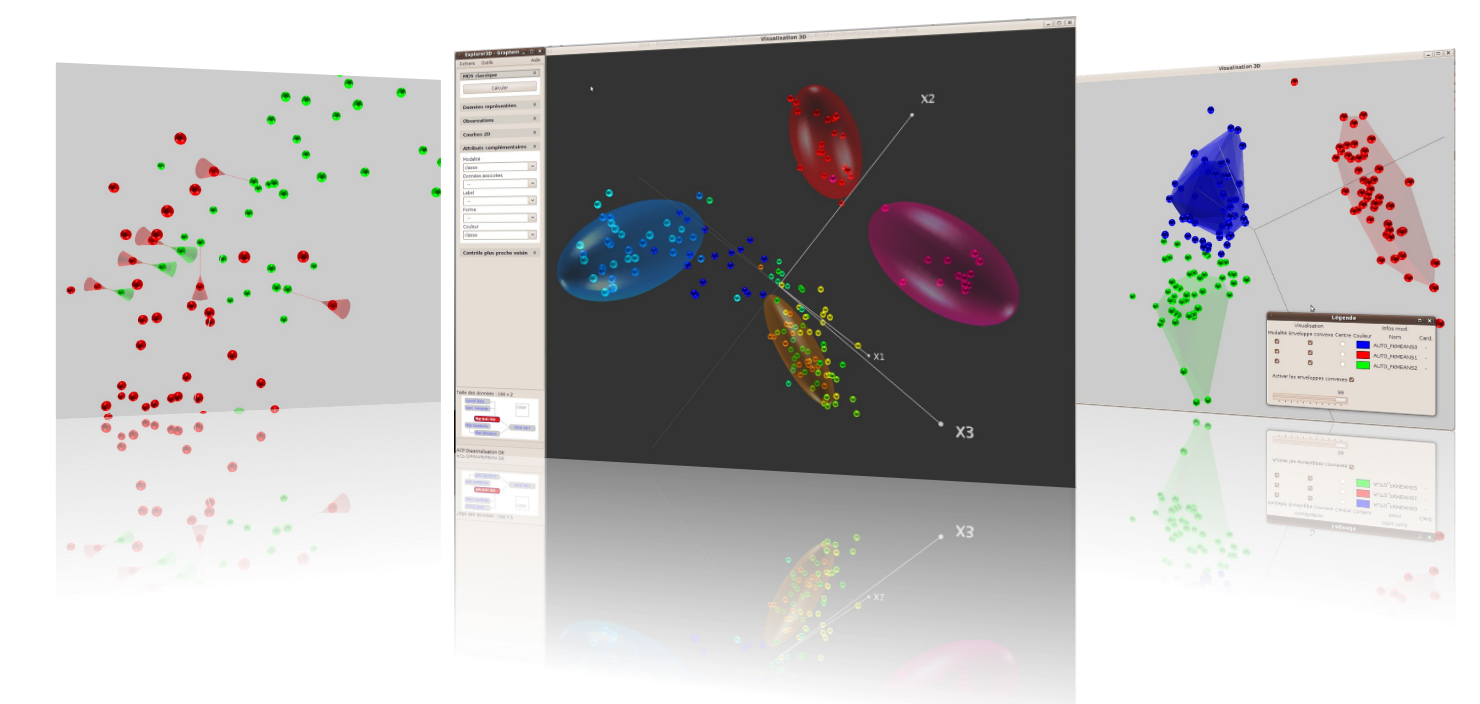
\includegraphics[scale=0.3]{explorer.png}\\
\textit{Les possibilités d'Explorer3D}
\end{center}


\newpage
\subsection{Packages R utilisables}
\paragraph{} Après quelques recherches sur internet, il apparaît qu'il existe des packages R, bibliothèques libres mise au point par la communauté, qui pourraient répondre à certains besoins du portage d'Explorer3D sous R. Nous en avons retenu deux pour le moment, RGL et Rgtk, qui semble répondre respectivement aux attentes en termes de : fenêtre 3D et interactions avec la scène 3D pour le premier, et interface utilisateur pour le second. Nous allons présenter plus en détails ces deux packages.
\subsubsection{RGL}
\paragraph{}
RGL est un package pour le langage de programmation R. Il étend les possibilités de R avec l'ajout d'outils de visualisation 3D en temps réel.
\paragraph{}
Les univers 3D ont besoin d’être projetées sur des images 2D affichées à l’écran, c'est pourquoi il est nécessaire d'avoir un outils qui effectue cette étape afin d'afficher des objets tri-dimensionnel à l’écran. Cet outils doit simuler la lumière, la structure des objets et leurs textures afin de donner l'illusion de 3D sur les images 2D projetées.
\begin{center}
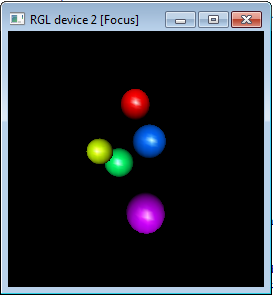
\includegraphics[scale=0.7]{screen_rgl2.png}\\
\textit{Des sphères dans RGL}
\end{center}


\paragraph{}
Le coeur de RGL est codé en c++ et utilise OpenGL. RGL est ainsi une interface entre R et OpenGL. OpenGL est un standard des applications graphiques utilisé dans un grand nombre d'applications et langages. Il résout notamment le problème d'affichage en 2D d'univers 3D cité plus tôt. 
\paragraph{}
Plusieurs fonctionnalités sont accessibles simultanément via RGL, telles que l’intégration drag/drop dans la fenêtre de visualisation et la réception de nouvelles instructions depuis la console de commande de R. Ainsi les objets peuvent être examinés en trois-dimension grâce au zoom et la scène peut pivoter sur elle-même.

\begin{center}
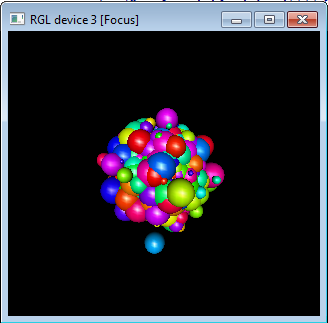
\includegraphics[scale=0.7]{screen_rgl3.png}\\
\textit{Plus de sphères dans RGL}
\end{center}


\paragraph{}
Le but de RGL est donc de surcoucher OpenGL pour le langage R. Il permet ainsi via des instruction en R de générer des scènes 3D et d'interagir avec celles-ci via de nombreux outils.

\newpage
\subsubsection{RGTK}
\paragraph{}
Le package RGtk2 s'ajoute en tant que librairie externe pour inclure dans R la possibilité de créer des interfaces graphiques. 

\paragraph{}
Comme dans Explorer3d, on a besoin de gérer les données grâce à l'interface graphique. Cette extension de R est essentielle dans le développement de l'application. 

 \begin{center}
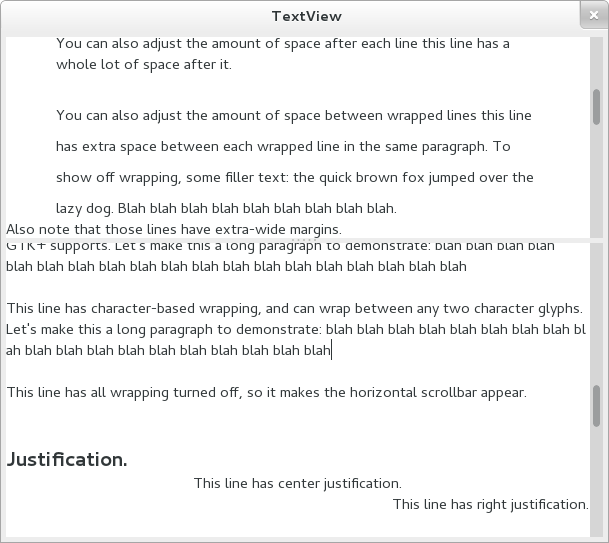
\includegraphics[scale=0.4]{multipleviews.png}\\
\textit{fenêtre divisée en plusieurs parties}
\end{center}

\paragraph{}
RGtk est un package dérivé de GTK2. Il est écrit en c++. GTK est un standard pour la création d'interface utilisateurs en c++ et bien d'autres langages. Grâce à RGtk2 nous pouvons résoudre le problème de création d'interface graphique. Comme dans la capture d’écran précédente nous pouvons créer une fenêtre avec plusieurs compartiments à l’intérieur de celle ci. Nous pouvons aussi avoir une fenêtre pour choisir la couleur d’un objet affiché dans une vue RG.

\begin{center}
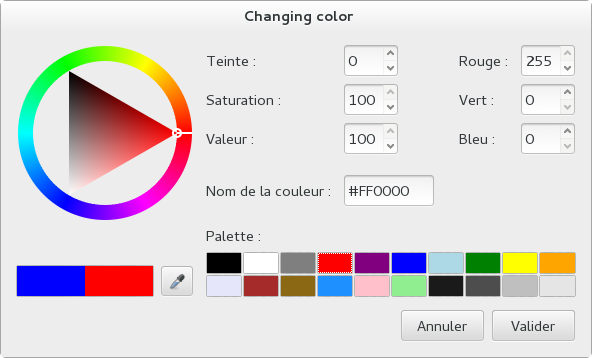
\includegraphics[scale=0.4]{colorselector2.png}\\
\textit{Sélectionneur de couleur RGtk}
\end{center}

\paragraph{}
Le but de RGtk2 est de surcoucher GTK. Avec ce package on pourra interagir avec le logiciel. \\\\\indent

Ce package nous offre la possibilité de créer
des interfaces graphiques pour l’utilisateur, ce qui lui permettra de faire les
demandes de calculs, sans passer par la console.\\

\begin{center}
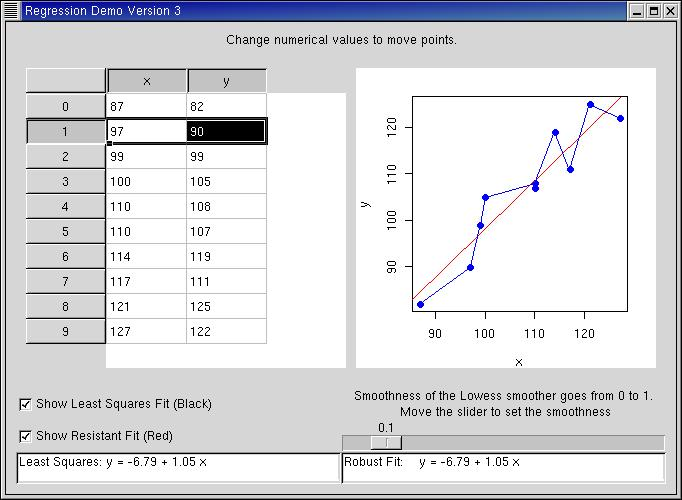
\includegraphics[scale=0.4]{regression.jpg}\\
\textit{Un autre exemple d'interface graphique avec RGtk}
\end{center}
\newpage